\documentclass[11pt]{article}
\usepackage{euscript}

\usepackage{amsmath}
\usepackage{amsthm}
\usepackage{amssymb}
\usepackage{mathtools}
\DeclarePairedDelimiter{\ceil}{\lceil}{\rceil}
\usepackage{epsfig}
\usepackage{xspace}
\usepackage{color}
\usepackage{url}
\usepackage{enumerate}
\usepackage{listings}

\usepackage{float}

%%%%%%%  For drawing trees  %%%%%%%%%
\usepackage{tikz}
\usetikzlibrary{calc, shapes, backgrounds}

%%%%%%%%%%%%%%%%%%%%%%%%%%%%%%%%%
\setlength{\textheight}{9in}
\setlength{\topmargin}{-0.600in}
\setlength{\headheight}{0.2in}
\setlength{\headsep}{0.250in}
\setlength{\footskip}{0.5in}
\flushbottom
\setlength{\textwidth}{6.5in}
\setlength{\oddsidemargin}{0in}
\setlength{\evensidemargin}{0in}
\setlength{\columnsep}{2pc}
\setlength{\parindent}{1em}
%%%%%%%%%%%%%%%%%%%%%%%%%%%%%%%%%

\newcommand{\eps}{\varepsilon}

\renewcommand{\c}[1]{\ensuremath{\EuScript{#1}}}
\renewcommand{\b}[1]{\ensuremath{\mathbb{#1}}}
\newcommand{\s}[1]{\textsf{#1}}

\newcommand{\E}{\textbf{\textsf{E}}}
\renewcommand{\Pr}{\textbf{\textsf{Pr}}}


\title{Asmt 2: Document Similarity and Hashing}
\author{Yulong Liang (u1143816)}

\begin{document}
\maketitle

\section{Creating $\textit{k}-$Grams (40 points)}

\paragraph{A: (20 points)}
Number of distinct k-grams for each document is as follows,
\begin{table}[h]
\centering
\begin{tabular}{c|c|c|c}
Document & G1 & G2 & G3\\
\hline
D1 & 263 & 765 & 279\\
D2 & 262 & 762 & 278\\
D3 & 269 & 828 & 337\\
D4 & 255 & 698 & 232\\
\end{tabular}
\end{table}

\paragraph{B: (20 points)}
Jaccard similarity between all pairs of documents is as follows,
\begin{table}[h]
\centering
\begin{tabular}{c|c|c|c}
Jaccard & G1 & G2 & G3\\
\hline
JS(1,2) & 0.981 & 0.978 & 0.941 \\
JS(1,3) & 0.816 & 0.580 & 0.182 \\
JS(1,4) & 0.644 & 0.305 & 0.030 \\
JS(2,3) & 0.800 & 0.568 & 0.174 \\
JS(2,4) & 0.641 & 0.306 & 0.030 \\
JS(3,4) & 0.653 & 0.312 & 0.016 \\
\end{tabular}
\end{table}

\section{Min Hashing (30 points)}

\paragraph{A: (25 points)}
The estimated Jaccard similarities are as follows,
\begin{table}[h]
\centering
\begin{tabular}{c|c}
t & Jaccard Similarity\\
\hline
20 & 0.98250 \\
60 & 0.97917 \\
150 & 0.98433 \\
300 & 0.97817 \\
600 & 0.97942 \\
\end{tabular}
\end{table}

\paragraph{B: (5 point)}
I ran Min Hashing Algorithm for \textbf{20 times} for each value of $t=\{20, 60, 150, 300, 600\}$ and calculated the \textbf{average value} of Jaccard Similarity between D1 and D2, Error between actual and estimated Jaccard Similarity, and the Run Time respectively.\\
\begin{table}[h]
\centering
\begin{tabular}{c|c|c|c|c}
t & Actual JS & Estimated JS & Error & Run Time\\
\hline
20 & 0.97798 & 0.98250 & 0.02411 & 0.08507 \\
60 & 0.97798 & 0.97917 & 0.01524 & 0.24098 \\
150 & 0.97798 & 0.98433 & 0.00841 & 0.56241 \\
300 & 0.97798 & 0.97817 & 0.00583 & 1.10425 \\
600 & 0.97798 & 0.97942 & 0.00469 & 2.28120 \\
\end{tabular}
\end{table}
As we increase the size of hash family, the error decreases whereas the run time increases. Thus we need to consider the trade-off and find a balance point. As shown in the chart below, I would pick the elbow point at around \texttt{t=150}.
\begin{figure}[H]
\centering{
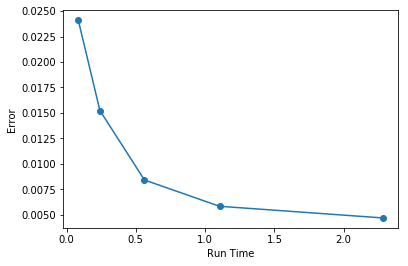
\includegraphics[width=.6\linewidth]{minhash.png}
}
\caption{Change of Error and Run Time with the Size of Hash Family}
\label{fig:name}
\end{figure}

\section{LSH (30 points)}

\paragraph{A: (8 points)}
Using the trick, $b$ and $r$ can be calculated as follows,
$$b\approx-\log_{0.7}160\approx14$$
$$r\approx\frac{t}{b}\approx11$$
However, this trick is only "rule of thumb". After plotting the relationship between $s$ and $f(x)$ regarding to all the possible value pairs around $b$ and $r$ above, we can find something different.
\begin{figure}[H]
\centering{
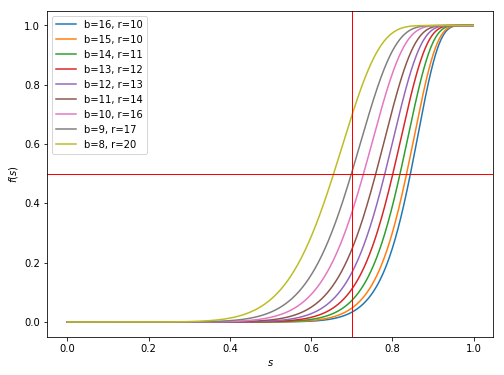
\includegraphics[width=.8\linewidth]{lshhash.png}
}
\caption{Relationship between $s$ and $f(s)$ with different value pairs of $b$ and $r$}
\label{fig:name}
\end{figure}
From the chart above, in order that $f(s)$ is close to 1 if $s>\tau$ and $f(s)$ is close to 0 if $s<\tau$, we want to have the curve steepest at $\tau=0.7$. \\\\
If we can use slightly less functions than 160 (which is 153), we want to pick the \textbf{grey curve} and the best value should be,
$$b=9$$
$$r=17$$
If we have to use up all the 160 functions, we want to pick the \textbf{pink curve} and the best value should be,
$$b=10$$
$$r=16$$
I will use $b=10$, $r=16$ in the following quesiton.

\paragraph{B: (22 points)}
For every pair of document, knowing the Jaccard Similarities from 1B, use the formula 
$$f(s)=1-(1-s^b)^r=1-(1-s^{10})^{16}$$ 
to calculate the probability of each pair being estimated to have similarity greater that $\tau=0.7$. The values are as follows,
\begin{table}[h]
\centering
\begin{tabular}{c|c|c|c|c}
Pair & JS & $Pr[similar]$\\
\hline
(D1,D2) & 0.97800 & 1.00000 \\
(D1,D3) & 0.58000 & 0.06675 \\
(D1,D4) & 0.30500 & 0.00011 \\
(D2,D3) & 0.56800 & 0.05448 \\
(D2,D4) & 0.30600 & 0.00012 \\
(D3,D4) & 0.31200 & 0.00014 \\
\end{tabular}
\end{table}

\newpage
\section{Appendix}
The code I used is as follows,
\begin{lstlisting}[language=Python]
import pandas as pd

import random
import string
import hashlib
import numpy as np
import time

import math
import numpy as np

from matplotlib import pyplot as plt

d = []
for i in range(1,5):
    with open('D'+str(i)+'.txt', 'r') as file:
        d.append(file.read())

char2gram = []
char2gram_size = []
for k in range(4):
    temp = set()
    for i in range(len(d[k])-1):
        temp.add(d[k][i:i+2])
    char2gram.append(temp)
    char2gram_size.append(len(temp))

char3gram = []
char3gram_size = []
for k in range(4):
    temp = set()
    for i in range(len(d[k])-2):
        temp.add(d[k][i:i+3])
    char3gram.append(temp)
    char3gram_size.append(len(temp))

word2gram = []
word2gram_size = []
for k in range(4):
    words = d[k].split()
    temp = set()
    for i in range(len(words)-1):
        temp.add(' '.join(words[i:i+2]))
    word2gram.append(temp)
    word2gram_size.append(len(temp))

def jaccard(set1, set2):
    return len(set1 & set2) / len(set1 | set2)

for i in range(0,4):
    for j in range(i+1, 4):
        js1 = jaccard(char2gram[i], char2gram[j])
        js2 = jaccard(char3gram[i], char3gram[j])
        js3 = jaccard(word2gram[i], word2gram[j])
        print('JS({0:d},{1:d}) & {2:.3f} & {3:.3f} & {4:.3f} \\\\'
        .format(i+1, j+1, js1, js2, js3))

t = [20, 60, 150, 300, 600]
k = t[0]

def randomsalt(k):
    salt = []
    for i in range(k):
        salt.append(''.join(random.choices(string.ascii_letters, k=10)))
    return salt

def inf2darray(k):
    v = []
    v.append([float('inf')] * k)
    v.append([float('inf')] * k)
    v.append([float('inf')] * k)
    v.append([float('inf')] * k)
    return np.array(v)

def jaccard_similarity(s1, s2):
    return sum(s1 == s2) / len(s1)

actual_js = jaccard(char3gram[0], char3gram[1])

result = {}
error = {}
runtime = {}
for k in t:
    sum_result = 0
    sum_error = 0
    sum_time= 0
    for n in range(20):
        start = time.time()
        salt = randomsalt(k)
        v = inf2darray(k)
        for d in range(2):
            for i in char3gram[d]:
                for j in range(k):
                    hashstr = hashlib.sha1((i+salt[j]).encode('utf-8'))
                    .hexdigest()
                    hashint = int(hashstr, 16) % 10000
                    if (hashint < v[d][j]):
                        v[d][j] = hashint
        pred_js = jaccard_similarity(v[0], v[1])
        sum_time += time.time() - start
        sum_result += pred_js
        sum_error += abs(actual_js - pred_js)
    result[k] = sum_result / 20
    error[k] = sum_error / 20
    runtime[k] = sum_time / 20

for key, value in result.items():
    print('{0:d} & {1:.5f} \\\\'.format(key, value))

for tt in t:
    print('{0:d} & {1:.5f} & {2:.5f} & {3:.5f} & {4:.5f} \\\\'
    .format(tt, actual_js, result[tt], error[tt], runtime[tt]))

plt.plot(runtime.values(), error.values(), 'o-')
plt.xlabel('Run Time')
plt.ylabel('Error')
plt.show()

def lsh(s, b, r):
    return 1 - (1 - s**b)**r

x = np.arange(0, 1, 0.001)

plt.figure(figsize=(8, 6))
plt.plot(x, lsh(x, 16, 10))
plt.plot(x, lsh(x, 15, 10))
plt.plot(x, lsh(x, 14, 11))
plt.plot(x, lsh(x, 13, 12))
plt.plot(x, lsh(x, 12, 13))
plt.plot(x, lsh(x, 11, 14))
plt.plot(x, lsh(x, 10, 16))
plt.plot(x, lsh(x, 9, 17))
plt.plot(x, lsh(x, 8, 20))
plt.axvline(x=0.7, linewidth=1, color='r')
plt.axhline(y=0.5, linewidth=1, color='r')
plt.legend(labels=['b=16, r=10',
                   'b=15, r=10',
                   'b=14, r=11',
                   'b=13, r=12',
                   'b=12, r=13',
                   'b=11, r=14',
                   'b=10, r=16',
                   'b=9, r=17',
                   'b=8, r=20'])
plt.xlabel(r'$s$')
plt.ylabel(r'$f(s)$')
plt.show()

b = 9
r = 17

js = np.array([0.978, 0.580, 0.305, 0.568, 0.306, 0.312])

for s in js:
    fx = (1 - (1 - s ** b)**r)
    print('{0:.5f} & {1:.5f}'.format(s, fx))
\end{lstlisting}

\end{document}
